%%---%% Physics Lab Report Version 0.6 - 1.febrúar 2023 %%---%%
% Höfundur/Author: Hákon Örn Árnason - hakona07 AT ru.is
% Viðhaldið af/Maintained by: Hákon Örn Árnason - hakona07 AT ru.is
%%%%%%%%%%%%%%%%%%%%%%%%%%%%%%%%%%%%%%%%%%%%%%%%%%%%%%%%%%%
% Credits to:
% Math template by Hlynur Arnarsson
% How to write text by Andrei Manolescu, Haraldur Auðunsson, Sigurður Ingi Erlingsson, version 050918
% Hákon Valur Haraldsson - figures and tables additions.
%%%%%%%%%%%%%%%%%%%%%%%%%%%%%%%%%%%%%%%%%%%%%%%%%%%%%%%%%%%

\documentclass{scrartcl}
% Skapalón frá Hlyni Arnórssyni
% Physics Version 0.2 - 10.Jan 2020
% ---------- Blaðsíðustillingar ---------- 
\usepackage{geometry}

\geometry{
	paper=a4paper, % letterpaper lika til
	top=2.5cm, % Top margin
	bottom=1cm, % Bottom margin
	left=2.5cm, % Left margin
	right=2.4cm, % Right margin
	headheight=0.75cm, % Header height
	footskip=1.5cm, % Space from the bottom margin to the baseline of the footer
	headsep=0.75cm, % Space from the top margin to the baseline of the header
	%showframe, % Uncomment to show how the type block is set on the page
}

% ---------- Íslenska ---------- 
\usepackage[T1]{fontenc}
\usepackage[utf8]{inputenc}
\usepackage[icelandic]{babel} % Setið 'english' í hornklofana ef skýrslan er alfarið á ensku.

% ---------- Stærðfræðipakkar frá AMS ---------- 

\usepackage{amsmath, amsfonts, amsthm, amssymb} % Stærðfræðipakkar
\usepackage{braket, nicefrac} % fyrir mengi, brotabrot

% ---------- Fyrir SI Einingar ---------- 
\usepackage{siunitx}

% ---------- Listar/ númeringar ---------- 
\usepackage{enumitem, multicol}

% ---------- Fyrir innsetningu mynda ---------- 
\usepackage{graphicx, float} 
\usepackage{keystroke}

% ---------- Til að teikna/tekka myndir ---------- 
\usepackage{tikz}
\usepackage{tkz-euclide}
\usetikzlibrary{math}
\usepackage{fourier}
\usetikzlibrary{quotes,angles}
\usepackage{tkz-euclide}
\usetikzlibrary{calc}
\usepackage[siunitx, nooldvoltagedirection]{circuitikz} %%<--- Circuit Diagrams/Rafrása myndir
\usepackage{csquotes}
%%%%%%%%%%%%%%%%%%%%%%%%%% Hyperlink References %%%%%%%%%%%%%%%%%%%%%%%%%%%
\usepackage[colorlinks=true, linkcolor=blue, citecolor=blue, urlcolor=blue, bookmarks=true, breaklinks=true]{hyperref}
\labelformat{equation}{(#1)} %jöfnu fix
\def\equationautorefname#1{}%for autoref, gobble the space
%%%%%%%%%%%%%%%%%%%%%%%%%%
% ---------- Nýtt Matlab viðmót ---------- 
\usepackage{listings}
\usepackage{fancyvrb}

\def\lstbasicfont{\fontfamily{pcr}\selectfont\normalsize}
\definecolor{mygreen}{RGB}{28,172,0} 
\definecolor{mylilas}{RGB}{170,55,241}
\lstset{language=Matlab,%
	basicstyle={\lstbasicfont},
	breaklines=true,%
	morekeywords={matlab2tikz},
	keywordstyle=\color{blue},%
	morekeywords=[2]{1}, keywordstyle=[2]{\color{black}},
	identifierstyle=\color{black},%
	stringstyle=\color{mylilas},
	commentstyle=\color{mygreen},%
	showstringspaces=false, %without this there will be a symbol in the places where there is a space
	numbers=left,%
	numberstyle={\tiny \color{black}},% size of the numbers
	numbersep=5 pt, % this defines how far the numbers are from the text 
	inputencoding=latin1,
	backgroundcolor = \color{gray!3},
	framexleftmargin= -1 mm,
	frame=none,
	rulesepcolor=\color{blue!30},
	extendedchars=true,
	emph={logical},emphstyle=\color{blue},	
	emph={all,equal, minor, on, off, long, short, bank, rat},emphstyle=\color{mylilas},	
}
\renewcommand\lstlistingname{\textsc{Matlab}}%

\usepackage{tcolorbox}
\tcbuselibrary{skins}
% ---------- Hérna vel ég stillingar fyrir ramma sem ég skýri matlabUT
\tcbset{matlabUT/.style={
		enhanced,
		colback=gray!1,
		colframe=gray!30,
		title=Command Window,
		arc=0mm,
		coltitle=black,
		center title, 
		title style={top color=white, bottom color = gray!30},
		grow to left by= -3 mm,
		left= 4 mm,
		grow to right by=0.5mm,
		colupper = gray!70!black
}}

%  ---------- Les inn textaskra sem inniheldur niðurstöður úr Command Window
\newcommand{\CommandWindow}[1]{\begin{tcolorbox}[matlabUT]
		\VerbatimInput{#1}
\end{tcolorbox}}


%%%%%%%%%%%%%%%% Matlab endar %%%%%%%%%%%%%%%%%%%%%%%%%%%%%%%%%%%%%%%%

%%%%% Geogebra  %%%%%%%%%%%%%%%%%%%%%%%%%%%%%%%%%%%%%%%%%%%%%%%%%
% ---------- Nokkur tól í GeoGebru, smíða einnig skurðtólið ---------- 

\newcommand{\Punktur}{% Punktur í GeoGebru
	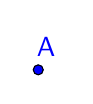
\begin{tikzpicture}[scale = 2]
	\draw
	(0,0) coordinate(A)
	(0.05,0.025) coordinate(pos)
	node[blue, anchor = south] {$\mathsf{A}$}  
	[blue,fill](A) circle(0.85pt); 
	\draw      [color = black](A) circle(0.9pt);
	\end{tikzpicture}
}
\newcommand{\Linustrik}{%  Strik, segment
	
\begin{tikzpicture}[scale = 0.4]
	\draw
	(0,0) coordinate(A)
	(1,0.7) coordinate(B)
	[line width = 1pt, blue](A)--(B);
	\draw[blue, fill](A) circle(4pt);
	\draw[blue, fill](B) circle(4pt);
	\end{tikzpicture}	
}

\newcommand{\Lina}{% bein lína, hægt að framlengja að vild
	
\begin{tikzpicture}[scale = 0.5]
	\draw
	(0,0) coordinate(A)
	(1,0.7) coordinate(B)
	[line width = 1pt, blue](A)--(B);
	\draw[blue, fill](0.25,0.18) circle(3pt);
	\draw[blue, fill](0.74,0.53) circle(3pt);
	\end{tikzpicture}	
}
\newcommand{\Halflina}{% við smíð á hornum
	
\begin{tikzpicture}[scale = 0.4]
	\draw
	(0,0) coordinate(A)
	(1,0.7) coordinate(B)
	[line width = 1pt, blue](A)--(B);
	\draw[blue, fill](A) circle(3pt);
	\draw[blue, fill](0.65,0.45) circle(3pt);
	\end{tikzpicture}	
	
}

\newcommand{\GeoO}{
	\begin{tikzpicture}[rotate=30,transform canvas={scale=0.18},yshift=7mm]
	\def\xrad{0.7}
	\def\yrad{0.58}
	\definecolor{GeogebraLitur}{rgb}{0.6,0.60,100}
	\tikzset{hnutur/.style={shape=circle, line width=0.7mm,color=black, fill=GeogebraLitur, scale=0.8, draw}} % 0.8
	\draw[ color = gray!70!black, line width=1.3mm] (0,0) circle[x radius = \xrad cm, y radius = \yrad cm];
	\def\n{5}
	\foreach \k in {1,...,\n}
	\node at ({360/\n*\k-10}:\xrad cm and \yrad cm)[hnutur] {};
	%	node[pos=1,hnutur]{} ;
	\end{tikzpicture}
}
\newcommand{\Geogebra}{{\color{gray!70!black}\textsf{Ge}\ \GeoO\textsf{Gebra }}}




% ---------- Skrá fyrir myndir ---------- 
\graphicspath{{graphics/}{Graphics/}{./}}
% ---------- Skrá fyrir heimildir ---------- 
\usepackage[style=ieee]{biblatex}
\addbibresource{bibliography.bib}
\usepackage{mathtools}
\begin{document}

%% --- Titil síða / Title page --- %%
\begin{titlepage}
	\centering
	
\includegraphics[width=0.3\textwidth]{LOGO.PNG}\par\vspace{1cm} %<-- RU Logo
	{\scshape\LARGE Indian Institute of Technology, Bombay \par} %<-- Nafn háskólans (Háskólinn í Reykjavík / Reykjavik University)
	\vspace{1cm}
	{\scshape\Large EE338 - Digital Signal Processing \par} %<-- Áfanga titill / Class or course title
	\vspace{1.5cm}
	{\huge\bfseries Digital Filter design\par} %<-- Titill Skýrslu / Title of Report
	\vspace{2cm}
	{\Large\itshape Name}\par %<-- Nafn nemanda / Name of student
	\texttt{Tejaswee Sulekh}\par %<-- t-póstfang / e-mail
	\vspace{0.7cm}
	{\Large\itshape Roll Number}\par %<-- Nafn nemanda / Name of student
	\texttt{20D070082}\par %<-- t-póstfang / e-mail
	\vfill
	Reviewed by\par %<-- (Umsjón höfðu / supervised by)
	   Hemant Hajare, 20D070037 %<-- Nafn kennara og aðstoðarkennara í tilraun / Name of Lab Teacher and TA
	\vfill

% Bottom of the page
	{\large Group Number-26\par}
\end{titlepage}

%% --- Titil síða endar / Title page ends --- %%

\section{FIR filter transfer function using Kaiser Window}

\subsection{Bandpass Filter}
The tolerance for both the stopband and passband is given to be $\delta = 0.15$ and we get the minimum stopband attenuation as
\begin{equation}
    A = - 20log_{10}(\delta) = -16.4782 dB
\end{equation}

Since A $\leq$ 21 we get $\beta$ to be 0 where $\beta$ is the shape parameter of the Kaiser window.
In order to estimate the required window length, we use the empirical formula for the lower bound on the window length.

\begin{equation}
    N_{min} = \frac{A - 8}{2.285\times2\times\Delta\omega_{T}}
\end{equation}

Here $\omega_{T}$ is the minimum transition width from the stopband to the passband.

\begin{equation}
    \Delta\omega_{T} = \frac{5kHz\times2\times\pi}{600kHz} = 0.0167\pi
\end{equation}

Substituting $\Delta\omega_{T}$ we get $N_{min} = 71$

The above equation gives a loose bound on the window length when the tolerance in not very stringent. From trial and error in MATLAB and checking if the specific given for the filter that I had to design the window length after this was $\textbf{96}$. The window is a rectangular window as $\beta = 0$.\\

The time domain coefficients were obtained by first generating the ideal impulse response samples for the same length as that of the window. The Kaiser window was generated using the MATLAB function and applied  on the ideal impulse response. The ideal impulse response was generated using a linear combination of impulse response of the ideal lowpass filter. The cutoff value and number of samples were given as the input argument to the ideal lowpass filter generating function.\\

\begin{figure}[ht!]
    \centering
    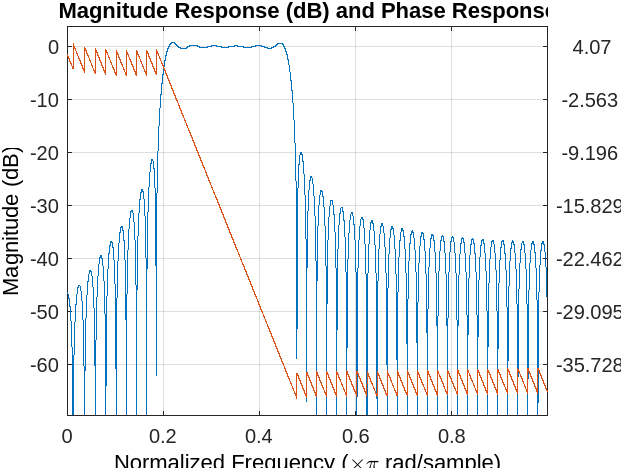
\includegraphics[width = 0.8\textwidth]{Graphics/MagPhaseBandpass.png}
    \caption{Magnitude Phase Response}
\end{figure}

\begin{figure}[ht!]
    \centering
    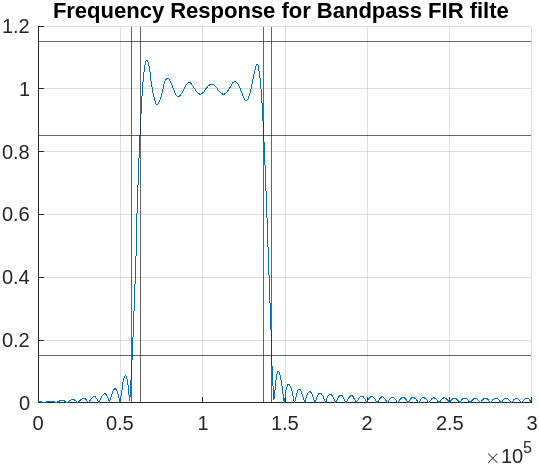
\includegraphics[width = 0.85\textwidth]{Graphics/BandpassFIR.png}
    \caption{Frequnecy Response}
\end{figure}

\begin{figure}[ht!]
    \centering
    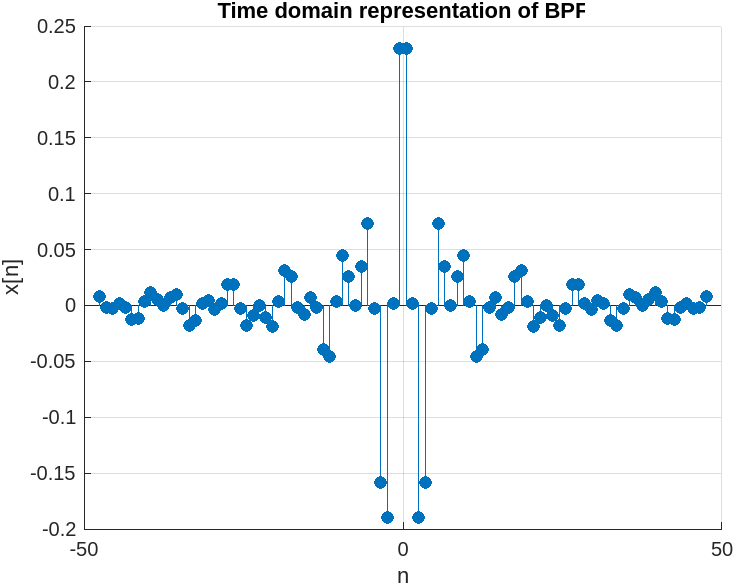
\includegraphics[width = 0.85\textwidth]{Graphics/impulsepass.png}
    \caption{Impulse Response}
\end{figure}

\begin{figure}[ht!]
    \centering
    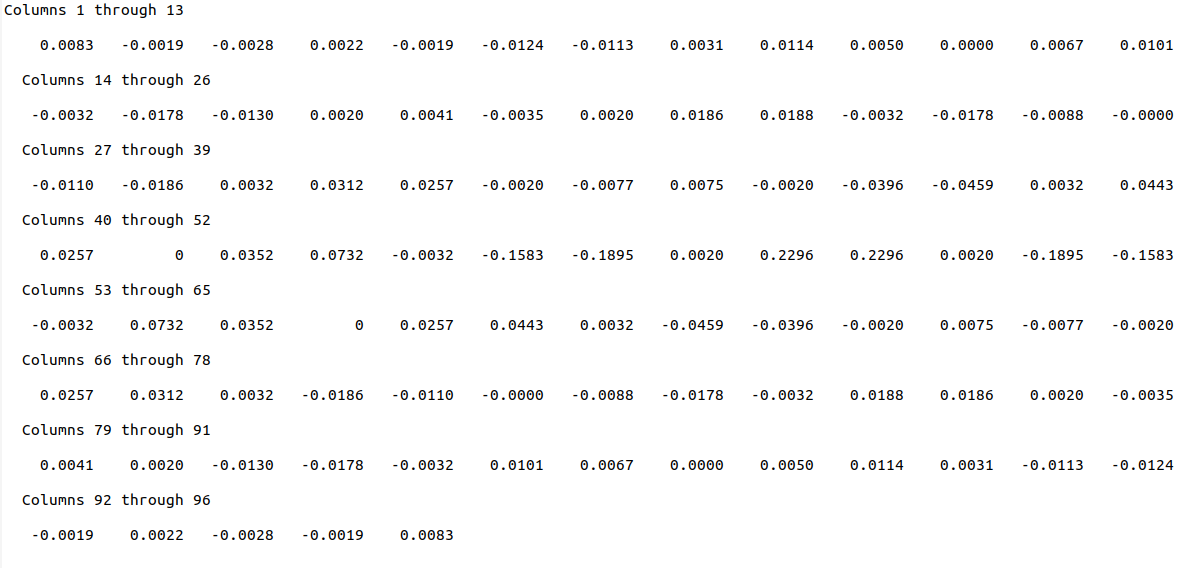
\includegraphics[width = 0.85\textwidth]{Graphics/BandpassCol.png}
    \caption{Coefficients for discrete impulse response}
\end{figure}

\newpage
\subsection{Bandstop}
Since we have similar tolerance requirements as we had for bandstop. This means that we will get similar results for A and its corresponding $\beta$ value.

\begin{equation}
    A = - 20log_{10}(\delta) = -16.4782 dB
\end{equation}

Since A $\leq$ 21 we get $\beta$ to be 0 where $\beta$ is the shape parameter of the Kaiser window.
In order to estimate the required window length, we use the empirical formula for the lower bound on the window length.

\begin{equation}
    N_{min} = \frac{A - 8}{2.285\times2\times\Delta\omega_{T}}
\end{equation}

Here $\omega_{T}$ is the minimum transition width from the stopband to the passband.

\begin{equation}
    \Delta\omega_{T} = \frac{5kHz\times2\times\pi}{425kHz} = 0.0232\pi
\end{equation}

Substituting $\Delta\omega_{T}$ we get $N_{min} = 51$

The above equation gives a loose bound on the window length when the tolerance in not very stringent. From trial and error in MATLAB and checking if the specific given for the filter that I had to design the window length after this was $\textbf{67}$. The window is a rectangular window as $\beta = 0$.\\

The time domain coefficients were obtained by first generating the ideal impulse response samples for the same length as that of the window. The Kaiser window was generated using the MATLAB function and applied  on the ideal impulse response. The ideal impulse response was generated using a linear combination of impulse response of the ideal lowpass filter. The cutoff value and number of samples were given as the input argument to the ideal lowpass filter generating function.\\

\begin{figure}[ht!]
    \centering
    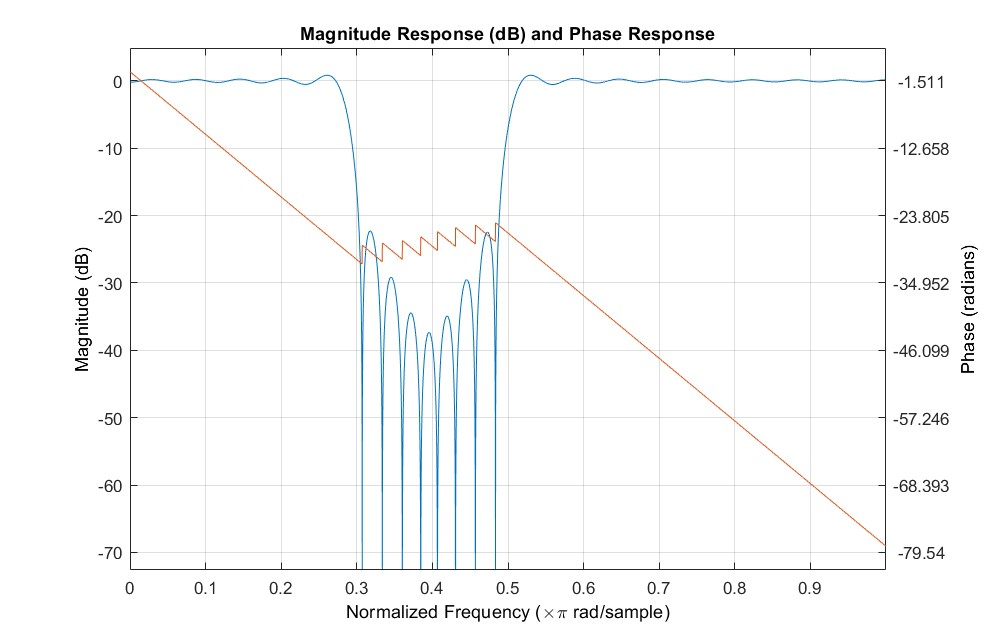
\includegraphics[width = \textwidth]{Graphics/Bandstop.jpg}
    \caption{Magnitude Phase Response}
\end{figure}

\begin{figure}[ht!]
    \centering
    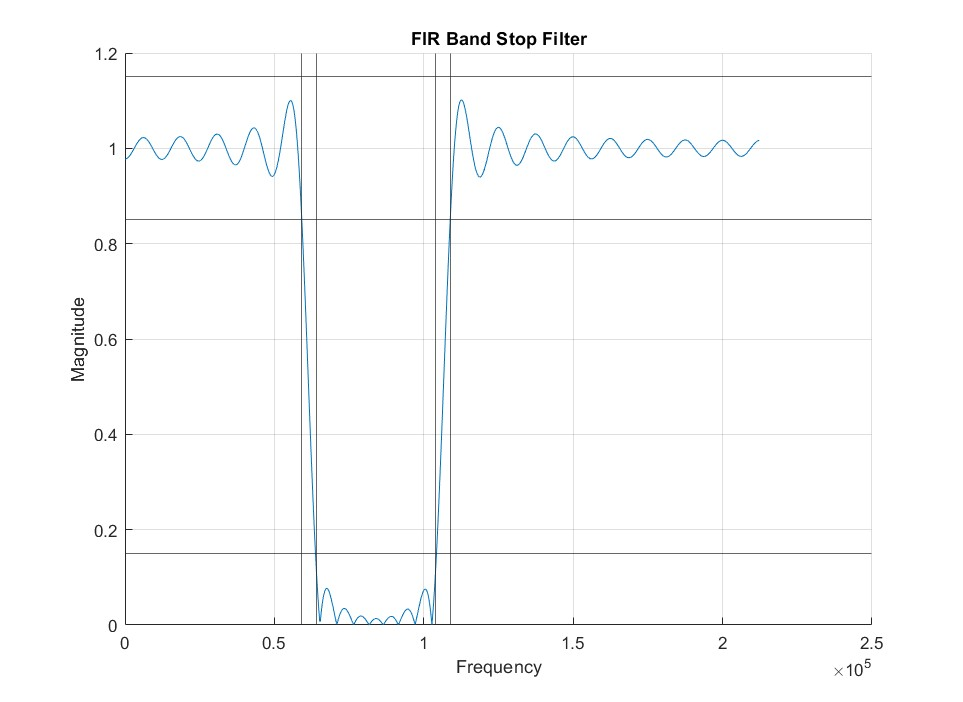
\includegraphics[width = \textwidth]{Graphics/Freq.jpg}
    \caption{Frequnecy Response}
\end{figure}

\begin{figure}[ht!]
    \centering
    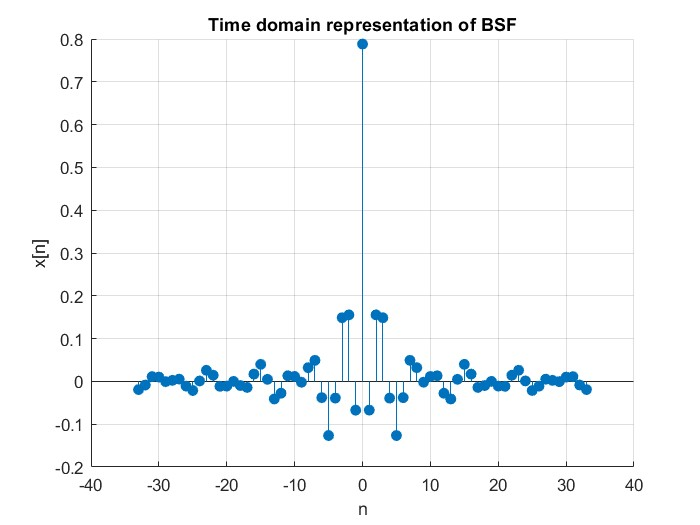
\includegraphics[width = 0.8\textwidth]{Graphics/Impulsestop.jpg}
    \caption{Impulse Response}
\end{figure}

\begin{figure}[ht!]
    \centering
    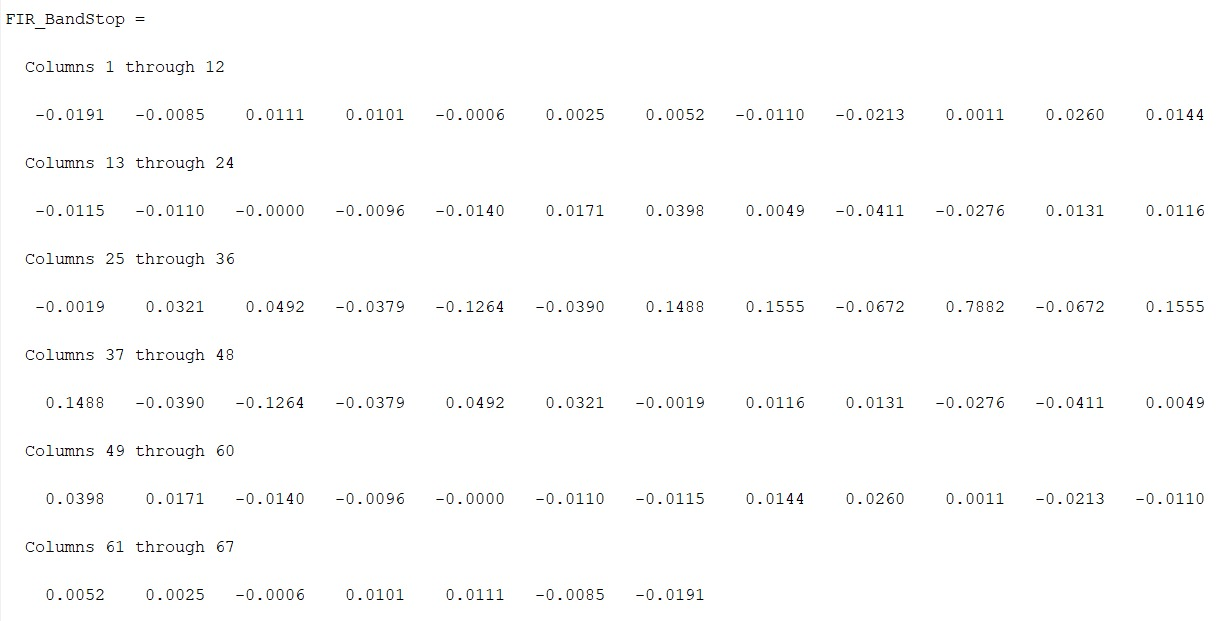
\includegraphics[width = 0.8\textwidth]{Graphics/Bandstopcol.jpeg}
    \caption{Coefficients for discrete impulse response}
\end{figure}
\newpage

\section{Peer Review Acknowledgement}

To whosoever it may concern, I have succesfully reviewed this filter design report done by Hemant Hajare as a part of this course assignment for EE338, Digital Signal Processing. This includes the design process, context, calculations, simulation program and results.\\
\\
Thank you,\\
Regards\\
Tejaswee Sulekh\\
20D070082\\


\end{document}